\documentclass{article}

\usepackage{fancyhdr}
\usepackage{amsmath}
\usepackage{amsthm}
\usepackage{amsfonts}
\usepackage{tikz}
\usepackage[plain]{algorithm}
\usepackage{algpseudocode}
\usepackage{graphicx}

\usetikzlibrary{automata,positioning}
\usepackage{listings}
\usepackage{xcolor}


%
% Basic Document Settings
%

\topmargin=-0.45in
\evensidemargin=0in
\oddsidemargin=0in
\textwidth=6.5in
\textheight=9.0in
\headsep=0.25in

\linespread{1.1}

\pagestyle{fancy}
\lhead{\hmwkAuthorName}
\chead{} % empty
\rhead{\hmwkHeaderTitle}
\cfoot{\thepage}

\renewcommand\headrulewidth{0.4pt}
\renewcommand\footrulewidth{0pt}

\setlength\parindent{0pt}

%
% Homework Details
%

\newcommand{\hmwkTitle}{[Ex3] Shell Scripting}
\newcommand{\hmwkDueDate}{Sunday, September 28, 2025,\ 11{:}59 pm (Thai time)}
\newcommand{\hmwkClass}{ICCS121 System Skills \& Low-Level Programming}
\newcommand{\hmwkClassTime}{(Section 2)}
\newcommand{\hmwkClassInstructor}{Songpon Teerakanok}
\newcommand{\hmwkAuthorName}{\textbf{Jiraroj Wiruchpongsanon (6781617)}}

% What appears in the top-right header
\newcommand{\hmwkHeaderTitle}{ICCS121 Sys Skills \& Low-Level Programming: Shell Scripting}

%
% Title Page
%

\title{
    \vspace{2in}
    \textmd{\textbf{\hmwkClass:\ \hmwkTitle}}\\
    \normalsize\vspace{0.1in}\small{Due\ on\ \hmwkDueDate}\\
    \vspace{0.1in}\large{\textit{\hmwkClassInstructor\ \hmwkClassTime}}
    \vspace{3in}
}

\author{\hmwkAuthorName}
\date{}

\renewcommand{\part}[1]{\textbf{\large Part \Alph{partCounter}}\stepcounter{partCounter}\\}

\lstset{
    basicstyle=\ttfamily\small,
    backgroundcolor=\color{gray!10},
    frame=single,
    breaklines=true,
    showstringspaces=false,
    keywordstyle=\color{blue},
    commentstyle=\color{green!50!black},
    stringstyle=\color{red!70!black}
}

%
% Helper Commands
%

\newcounter{partCounter}
\newcommand{\solution}{\textbf{\large Solution}}

\newtheorem*{theorem}{Theorem}

\theoremstyle{remark}
\newtheorem*{remark}{Remark}

\begin{document}

\maketitle
\newpage

\section*{File Organizer: Basic Folder Automation}

Students will write a bash script to organize files by extension into corresponding folders.

\medskip

\textbf{Tasks:}

\begin{enumerate}
    \item Setup:
    \begin{itemize}
        \item Create a folder named \texttt{unorganized/} and add 10 files of various types: i.e., \texttt{.txt}, \texttt{.jpg}, \texttt{.pdf}.
        \item Create and name 3 additional folders under the same parent directory: \texttt{images/}, \texttt{documents/}, and \texttt{texts/}.
    \end{itemize}

    \item Scripting: Create a script to move each file in \texttt{unorganized/} to its respective folder.
\end{enumerate}

\medskip

\textbf{Script Requirements:}

\begin{itemize}
    \item Loop through files in \texttt{unorganized/}.
    \item Create folders for each file extension if they don’t exist.
    \item Move files to the correct folder.
    \item For each file moved, print a one-line log on the screen. The log should look like the following:  
    \texttt{"Moving <filename> to <foldername>/"}
\end{itemize}

\medskip

\textbf{Sample screen output:}

\begin{verbatim}
===================================

Moving report.pdf to documents/
Moving image1.jpg to images/
Moving file1.txt to texts/
Organization Complete!

===================================
\end{verbatim}

\medskip

Note: The script must actually move the files to their respective folders, not just print the log.

\medskip
\newpage

\textbf{Deliverable:}

Students must submit a single PDF file containing the following:

\begin{enumerate}
    \item Bash Script (\texttt{setup.sh}):
    \begin{itemize}
        \item Paste the full script into the PDF.
        \item Ensure the script includes comments explaining each step.
    \end{itemize}
    \solution

    \begin{lstlisting}[language=bash, caption={organize.sh}]
    #!/bin/zsh

    # Setup:
    # Create a folder named unorganized/ and add 10 files of various types: i.e., .txt, .jpg, .pdf.
    # Create and name 3 additional folders under the same parent directory: images/, documents/, and texts/.

    # create `unorganized` directory
    mkdir ./unorganized/

    # array of various file types
    extensions=(txt log webp joblib pdf jpg wav arw tex csv json)

    # loop through `extensions` and create files
    for extension in $extensions; do
        touch "./unorganized/file.$extension"
    done

    # create `images/`, `documents/` and `texts/` directories as instructed
    mkdir ./images/
    mkdir ./documents/
    mkdir ./texts/
    \end{lstlisting}

    \begin{lstlisting}[language=bash, caption={organize.sh}]
    #!/bin/zsh

    # Scripting: Create a script to move each file in unorganized/ to its respective folder.

    # image extensions array
    image_extensions=(png jpg jpeg gif bmp tiff tif webp heic heif svg ico avif)

    # text extensions array
    text_extensions=(txt text log md markdown rtf tex rst cfg conf ini yaml yml json toml)

    # document extensions array
    document_extensions=(pdf doc docx odt rtf csv tsv xls xlsx ods ppt pptx odp)

    # Can't tolerate O(n) lookup time, so we change to hashmap
    typeset -A extensions_map=()

    # map extensions to image
    for extension in $image_extensions; do
        extensions_map[$extension]=image
    done 

    # map extensions to text
    for extension in $text_extensions; do
        extensions_map[$extension]=text
    done 

    # map extensions to document
    for extension in $document_extensions; do
        extensions_map[$extension]=document
    done 

    # Loop through files in unorganized/.
    for file in ./unorganized/*; do
        # i don't think we learn this in class -- i just google it; this should keep only string after `.`
        file_extension=${file##*.}
        # this one is similar to the ones above, just cut at the backmost `/` in file directory
        file_name=${file##*/}

        # '-z' prefix means missing/ don't exist
        if [[ -z ${extensions_map[$file_extension]} ]]; then
            # Create folders for each file extension if they don’t exist.
            mkdir ./$file_extension/
            # Move files to the correct folder.
            mv $file ./$file_extension/$file_name
            # For each file moved, print a one-line log on the screen. The log should look like the following: "Moving <filename> to <foldername>/"
            echo "Moving $file_name to ./$file_extension/"
        else
            case ${extensions_map[$file_extension]} in
                image)
                    # Move files to the correct folder.
                    mv $file ./images/$file_name
                    # For each file moved, print a one-line log on the screen. The log should look like the following: "Moving <filename> to <foldername>/"
                    echo "Moving $file_name to ./images/"
                    ;;
                text)
                    # Move files to the correct folder.
                    mv $file ./texts/$file_name
                    # For each file moved, print a one-line log on the screen. The log should look like the following: "Moving <filename> to <foldername>/"
                    echo "Moving $file_name to ./texts/"
                    ;;
                document)
                    # Move files to the correct folder.
                    mv $file ./documents/$file_name
                    # For each file moved, print a one-line log on the screen. The log should look like the following: "Moving <filename> to <foldername>/"
                    echo "Moving $file_name to ./documents/"
                    ;;
                *)
                    # panic, scream
                    echo "Ahhhhhhhhhhhhhhhhh!!!!!"
                    ;;
            esac
        fi
    done    
    \end{lstlisting}


    \item Before and After Screenshots:
    \begin{itemize}
        \item Before: Screenshot showing the \texttt{unorganized/} directory with mixed files.
        \item After: Screenshot showing organized folders (e.g., \texttt{texts/}, \texttt{images/}).
    \end{itemize}
    \solution

    \begin{figure}[h!]
        \centering
        \includegraphics[width=0.8\textwidth]{screenshot_before.png}
    \end{figure}

    \begin{figure}[h!]
        \centering
        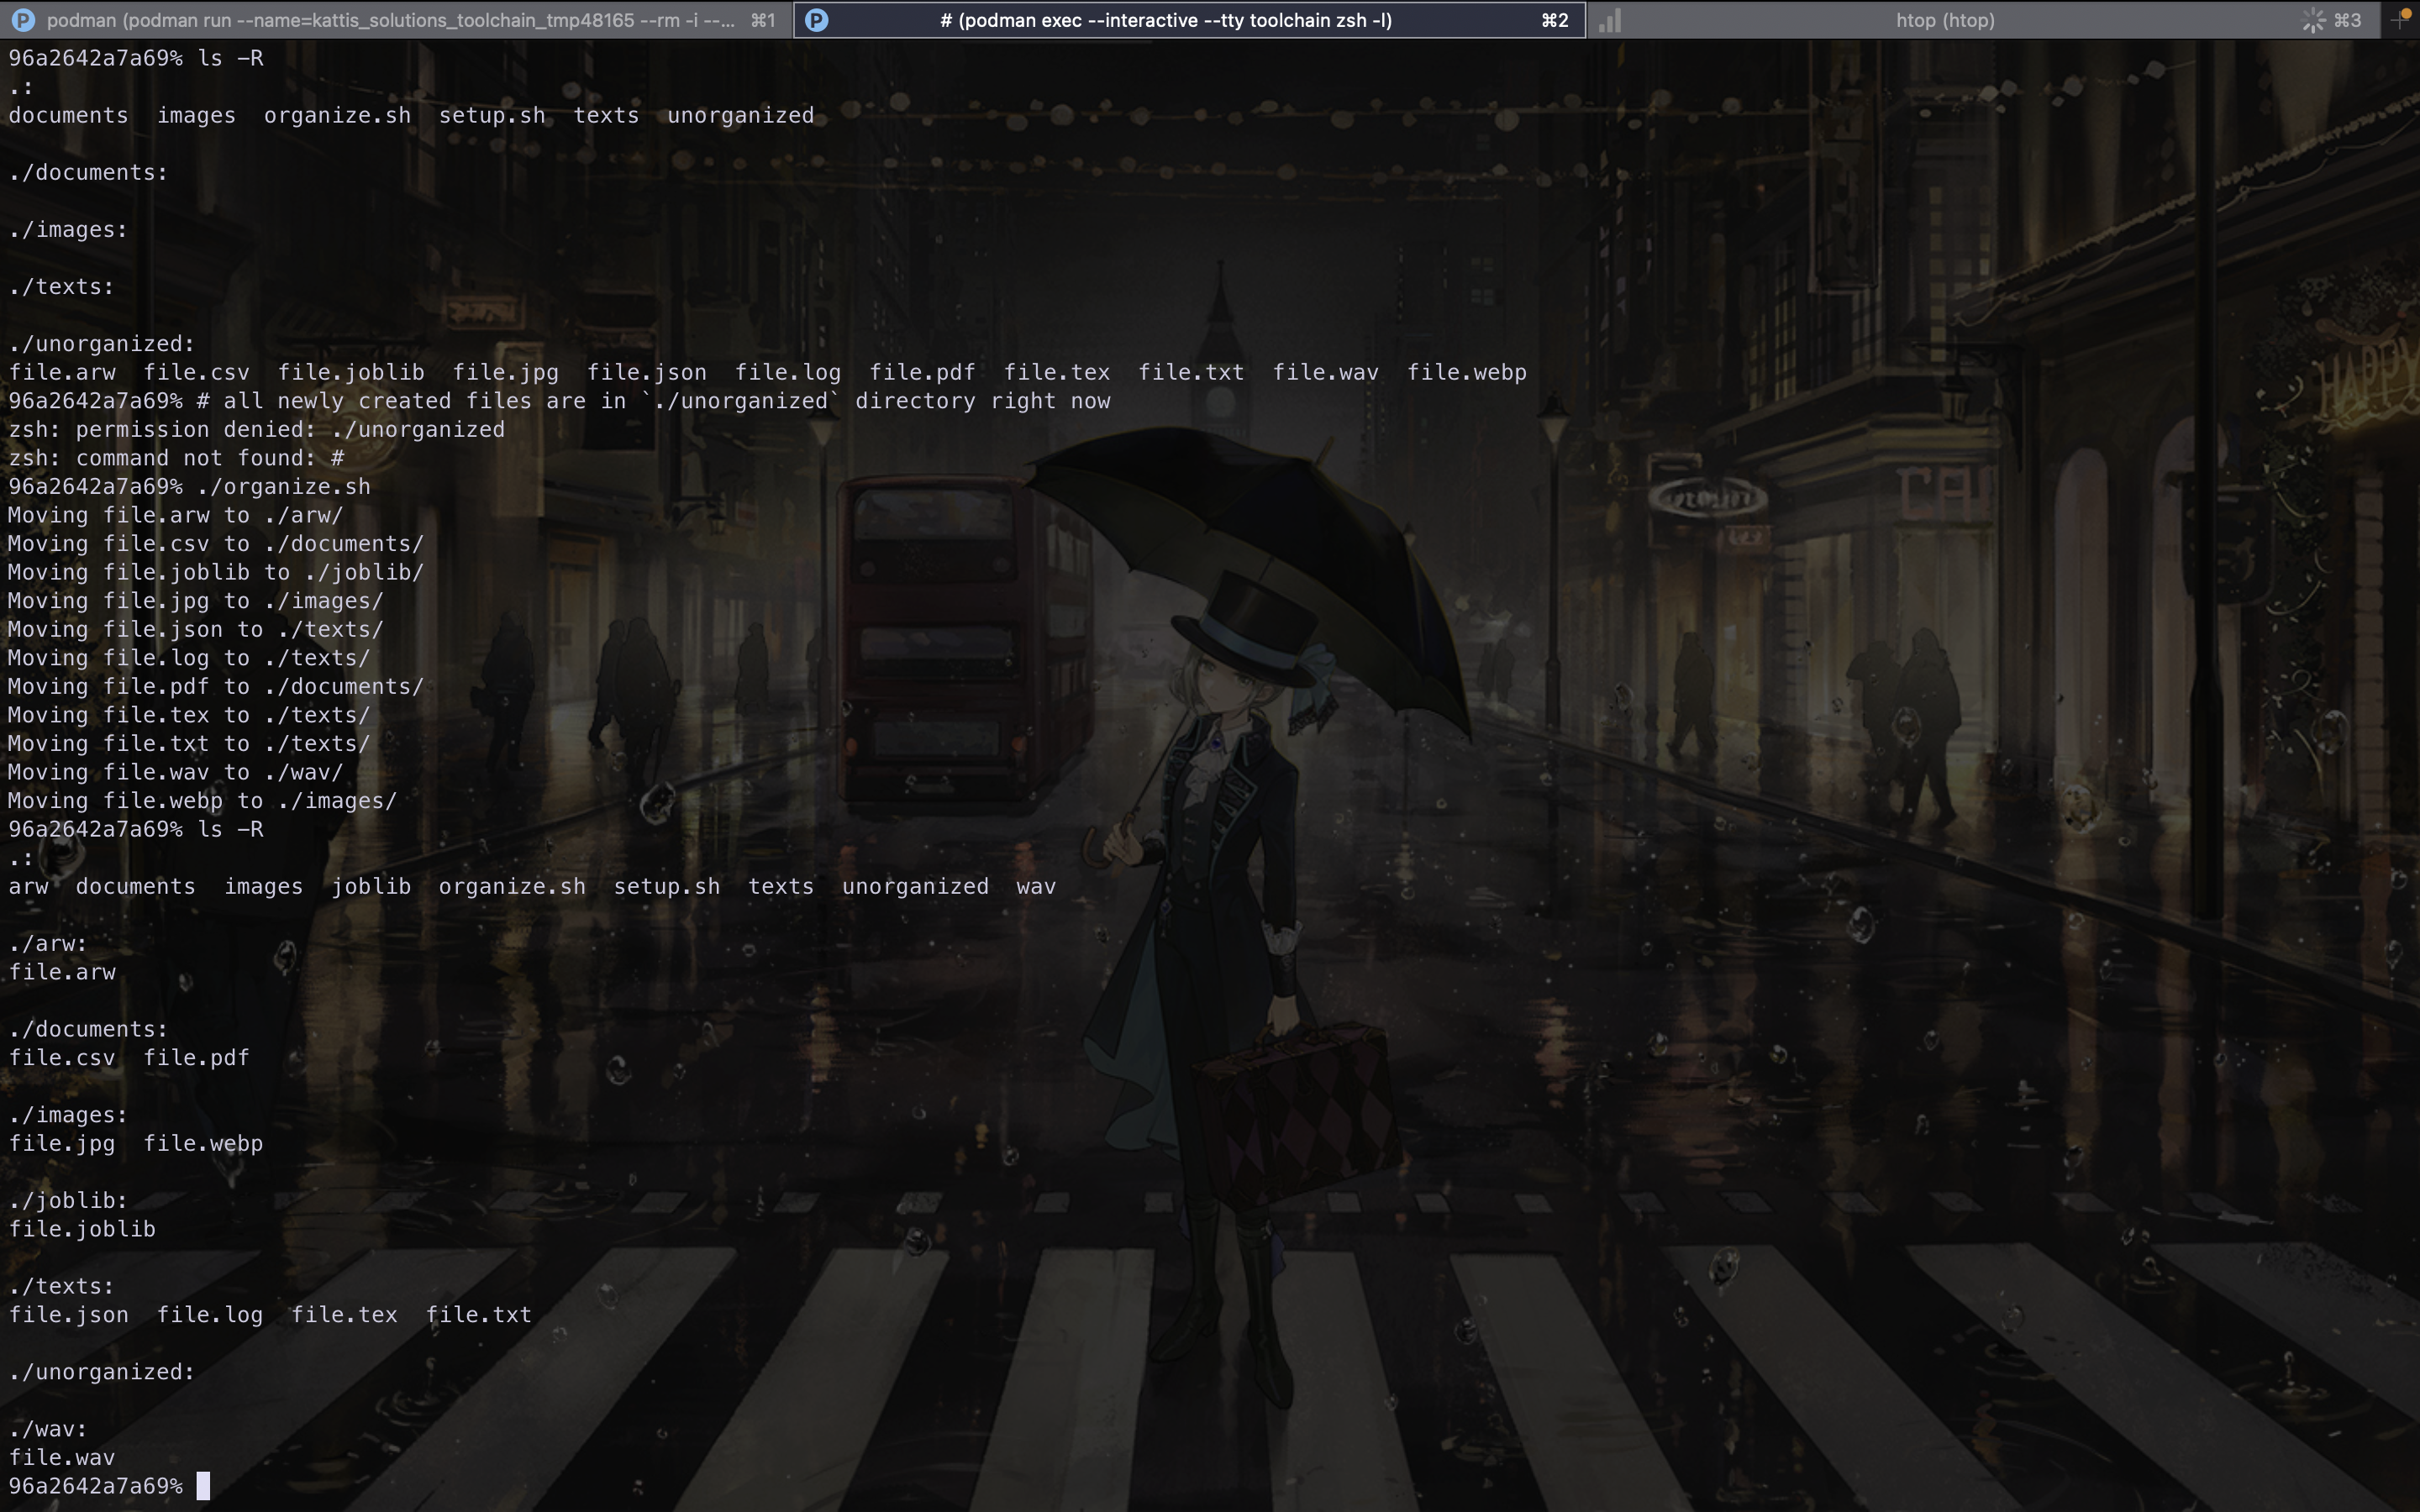
\includegraphics[width=0.8\textwidth]{screenshot_after.png}
    \end{figure}

    \item Sample Output (Log):
    \begin{itemize}
        \item Copy and paste the terminal output showing the log for each file moved.
    \end{itemize}
    \solution

    \begin{verbatim}
    96a2642a7a69% ./organize.sh 
    Moving file.arw to ./arw/
    Moving file.csv to ./documents/
    Moving file.joblib to ./joblib/
    Moving file.jpg to ./images/
    Moving file.json to ./texts/
    Moving file.log to ./texts/
    Moving file.pdf to ./documents/
    Moving file.tex to ./texts/
    Moving file.txt to ./texts/
    Moving file.wav to ./wav/
    Moving file.webp to ./images/
    \end{verbatim}

    \item Explanation:
    \begin{itemize}
        \item Write some sentences describing how the script works and the key commands used.
    \end{itemize}
    \solution

    Firstly, \textbf{\texttt{setup.sh}} sets up the environment as instructed (you can check that by the screenshot). 
    \textbf{\texttt{organize.sh}} organizes different file extensions into its place, else create a new directory for that unrecognised file. 
    We creates a hash map like structure first, for faster lookup time -- mapping file type (\textbf{key}) to its value (\textbf{destination folder}). 
    Then, we use that magical lines to get \textbf{\texttt{file\_extension}} and \textbf{\texttt{file\_name}} -- i don't think we learn this in class, I searched it up from google. 
    The rest is just checking whether the key matches or not and move the files to its destination.

    \end{enumerate}

\end{document}
